% !TeX spellcheck = en_US
% !TeX root = notes.tex
\section{Binary Arithmetic}
\subsection{Equivalent Circuits}
All circuits can be constructed from NAND and NOR gates

\subsection{Overflow}
Overflow with two's complement addition:
\begin{itemize}
	\item Carry into sign-bit is different to the carry out of the sign-bit
	\item Equivalently, overflow occurs if
	\subitem Two negatives added together give a positive, or
	\subitem Two positives added together give a negative	
\end{itemize}

\subsection{Full Adder}
\begin{figure}[H]
	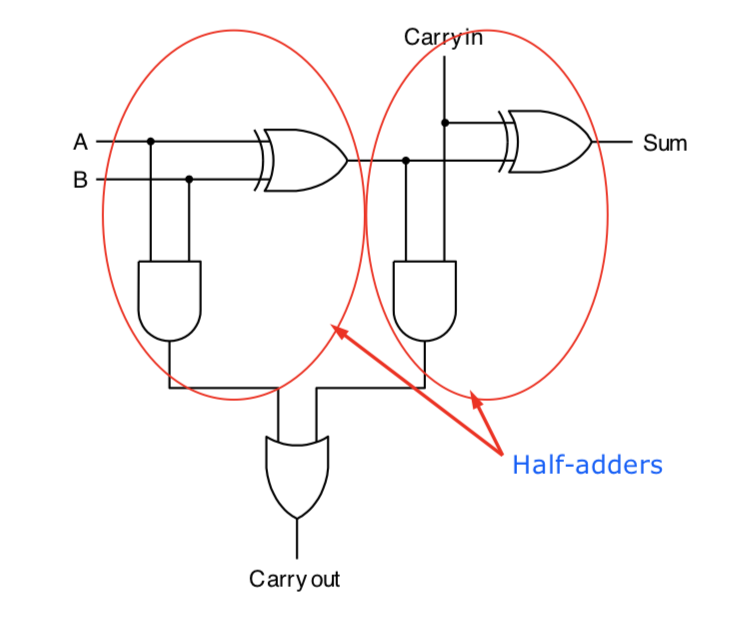
\includegraphics[width=0.8\linewidth]{fulladder}	
\end{figure}


\subsection{Binary Adder}
Can cascade full adders to make binary adder. This is a \textbf{ripple-carry adder}.
\begin{figure}[H]
	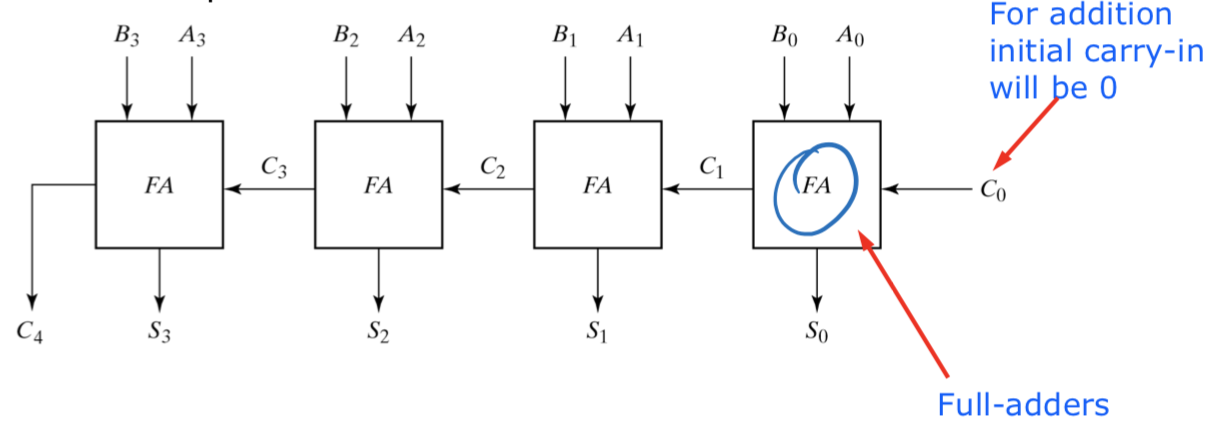
\includegraphics[width=0.8\linewidth]{binaryadder}	
\end{figure}



%\begin{circuitikz}
%	\draw (1, -2) node [and port,rotate=-90] (and1) {};
%	\draw (5, -2) node [and port,rotate=-90] (and2) {};
%	\draw (3, -4) node [or port,rotate=-90] (or1) {};
%	\draw (and1.out) |- (or1.in 2);
%	\draw (and2.out) |- (or1.in 1);
%	
%	\draw (3, 0.5) node [xor port] (xor1) {};
%	
%	\draw (0, 0) node (a) {A};
%	\draw (0, 1) node (b) {B};
%	
%	\draw (a) -| (and1.in 1);
%	\draw (a) -| (xor1.in 2);
%	\draw (b) -| (and1.in 2);
%	\draw (b) -| (xor1.in 1);
%\end{circuitikz}
